\documentclass[11pt]{article}

\newcommand{\cnum}{CM146}
\newcommand{\ced}{Fall 2018}
\newcommand{\ctitle}[3]{\title{\vspace{-0.5in}\cnum, \ced\\Problem Set #1: #2}}
\usepackage{enumitem}
\usepackage{graphicx}
\graphicspath{{/home/scott/Documents/Github/Machine_Learning/HW_3}}
\newcommand{\solution}[1]{{{\color{black}{\bf Solution:} {#1}}}}
\usepackage[usenames,dvipsnames,svgnames,table,hyperref]{xcolor}

\renewcommand*{\theenumi}{\alph{enumi}}
\renewcommand*\labelenumi{(\theenumi)}
\renewcommand*{\theenumii}{\roman{enumii}}
\renewcommand*\labelenumii{\theenumii.}


\begin{document}
\ctitle{3}{Computational Learning Theory, Kernel, SVM}
\author{Chaojie Feng}
\date{}
\maketitle
\vspace{-0.75in}

\section{Problem 1}

\solution{
The VC dimension is 3.
First of all, any cases of three points in the space can be shattered by this hypothesis space. This can be shown in the following figure 1 through figure 4. Note that there are $2^3 = 8$ possible configurations in total and I only select 4 of them. Just by switching the labels from original 4 examples will generate the other 4 examples.
	
	\begin{figure}[h!]
	\centering
	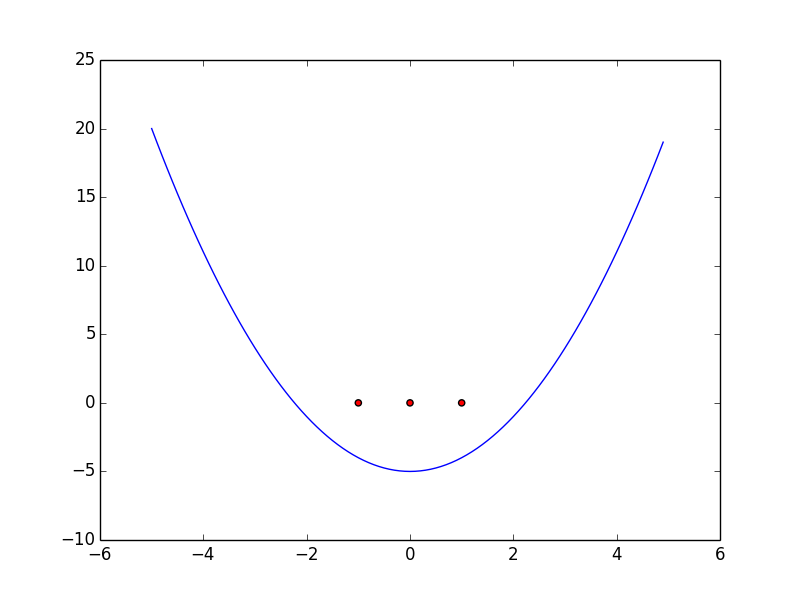
\includegraphics[width = 10cm]{1a}
	\caption{1st case of 3-point shattering}
	\end{figure}
	
	\begin{figure}[h!]
	\centering
	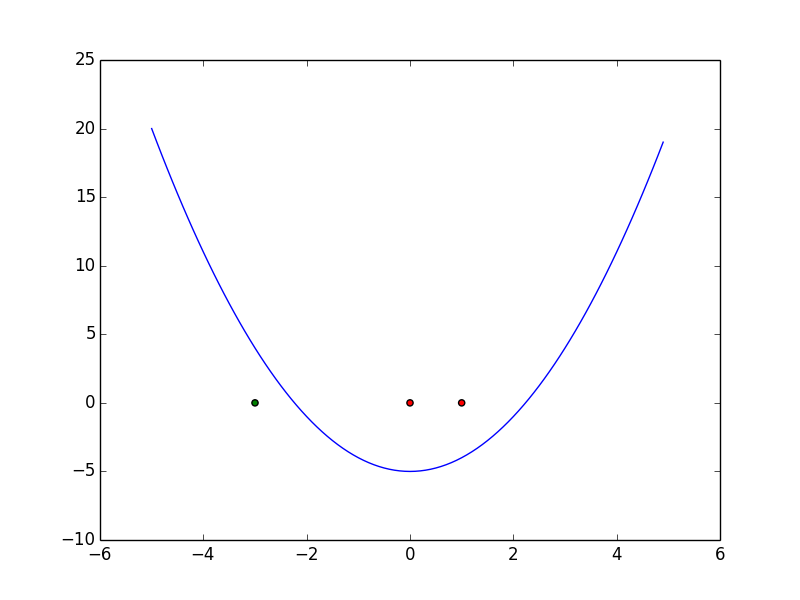
\includegraphics[width = 10cm]{1b}
	\caption{2nd case of 3-point shattering}
	\end{figure}
	
	\begin{figure}[h!]
	\centering
	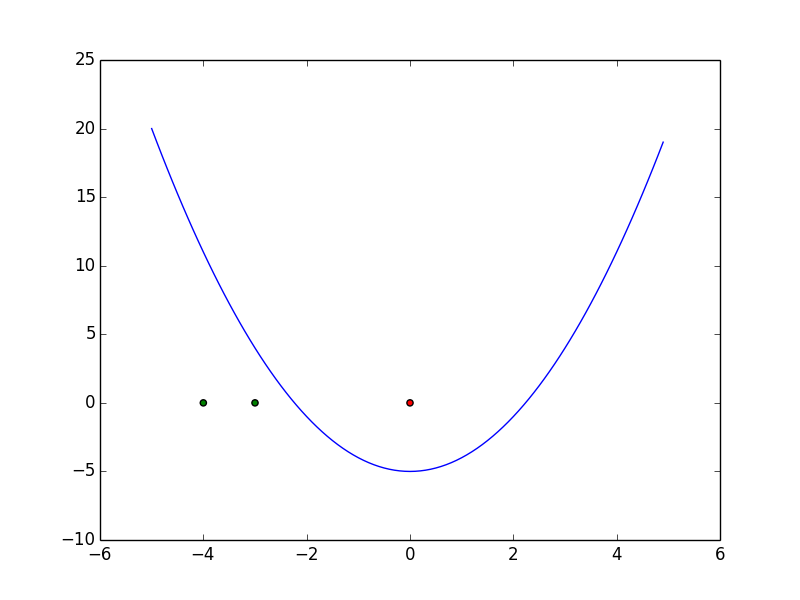
\includegraphics[width = 10cm]{1c}
	\caption{3rd case of 3-point shattering}
	\end{figure}
	
	\begin{figure}[h!]
	\centering
	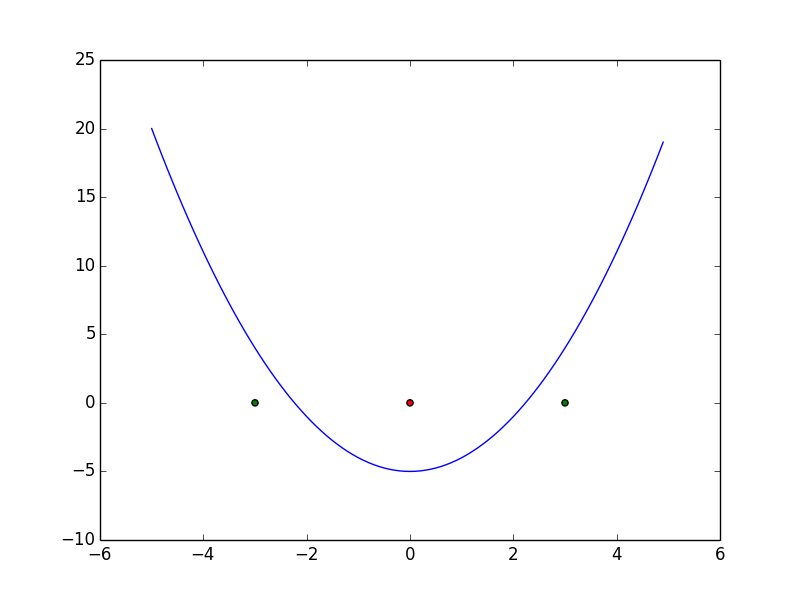
\includegraphics[width = 10cm]{1d}
	\caption{4th case of 3-point shattering}
	\end{figure}
	
However, this is not the case when there are four points in the space, 4-points cannot be shattered using this hypothesis space. As a result, $3 \leq VC(H) < 4$, $VC(H)$ = 3

	
	\begin{figure}[h!]
	\centering
	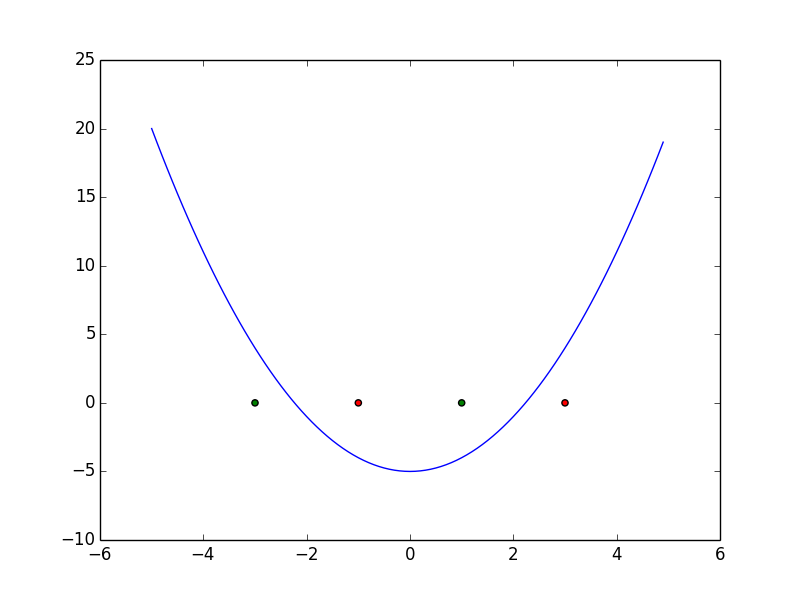
\includegraphics[width = 10cm]{1e}
	\caption{4-point shattering}
	\end{figure}
	
}

\vspace{5cm}

\newpage~\newpage~\newpage

\section{Problem 2}

\solution{From $(1+\beta x \cdot z)^3$, we can expand it as:

$$ 1+3\beta\sum_{d}^{D} x_dz_d + 3\beta^2\sum_{d}^{D}\sum_{e}^{D} x_dz_ex_ez_d +\beta^3\sum_{d}^{D}\sum_{e}^{D}\sum_{f}^{D} x_dz_dx_ez_ex_fz_f$$

It can be rather expanded and reformulated as:

$$ 1+3\beta\sum_{d}^{D} x_dz_d + 3\beta^2(\sum_{d}^{D}x_d^2z_d^2 + 2\sum_{d}^{D}\sum_{e\neq d}^{D}x_dz_dx_ez_e) + $$

$$ \beta^3(\sum_{d}^{D}x_d^3z_d^3 + 3\sum_{d}^{D}\sum_{e\neq d}^{D} + 6\sum_{d}^{D}\sum_{e\neq d}^{D}\sum_{f\neq d, e}^{D} x_dx_ex_fz_dx_ez_f)$$


We want to represent the above term as an inner product of two expanded feature vector $\phi_\beta(x)$

$$\phi_\beta(x) = [1, \sqrt{3\beta}x_1, \sqrt{3\beta}x_2, ...\beta\sqrt{3}x_1^2, \beta\sqrt{3}x_2^2.......$$

$$\beta\sqrt{6}x_1x_2, ...\sqrt{\beta^3}x_1^3, \sqrt{\beta^3}x_2^3 ... \sqrt{3\beta^3}x_1x_2^2...\sqrt{6\beta^3}x_1x_2x_3...]^T$$

In the same format, we can derive $\phi_\beta(z)$:

$$\phi_\beta(z) = [1, \sqrt{3\beta}z_1, \sqrt{3\beta}z_2, ...\beta\sqrt{3}z_1^2, \beta\sqrt{3}z_2^2.......$$

$$\beta\sqrt{6}z_1z_2, ...\sqrt{\beta^3}z_1^3, \sqrt{\beta^3}z_2^3 ... \sqrt{3\beta^3}z_1z_2^2...\sqrt{6\beta^3}z_1z_2z_3...]^T$$

Compared to $K(x, z) = (1+x \cdot z)^3$ (i.e. $\beta$ = 1), an additional $\beta$ can be tuned in the training process in order to fit the model better. So it provides more flexibility.



}

\vspace{5cm}
\newpage

\section{Problem 3}
\begin{enumerate}
\item Problem 3a

\solution{Since we only have two points $x_1$ and $x_2$ in 2D space, they must be points where SVM lies on. As a result, all of the inequalities must satisfy with equality in order to minimize the objective function:
$$ 1w(1, 1)^T = 1$$
$$ -1w(1, 0)^T = 1$$

Which suggests:
$$ w_1 + w_2 = 1$$
$$ -w_1 = 1$$}

As a result:
$$ w = (-1, 2)^T $$


\item Problem 3b

\solution{The procedure looks similar to problem 3a. In order to maximize margin, all of the inequalities must satisfy with equality:

$$ 1w(1, 1)^T + b = 1$$
$$ -1w(1, 0)^T +b= 1$$

$$ w_1 + w_2 + b = 1$$
$$ -w_1 - b= 1$$

$$ w_2 = 2 $$

In order to minimize objective function, $w_1 = 0$. As a result, $b = -1$. The solution is different from without offset term.
}

\end{enumerate}

\vspace{5cm}
\newpage

\section{Problem 4.1}

\begin{enumerate}

\item Problem 4.1(a)

\solution{
	
	
	\begin{figure}[h!]
	\centering
	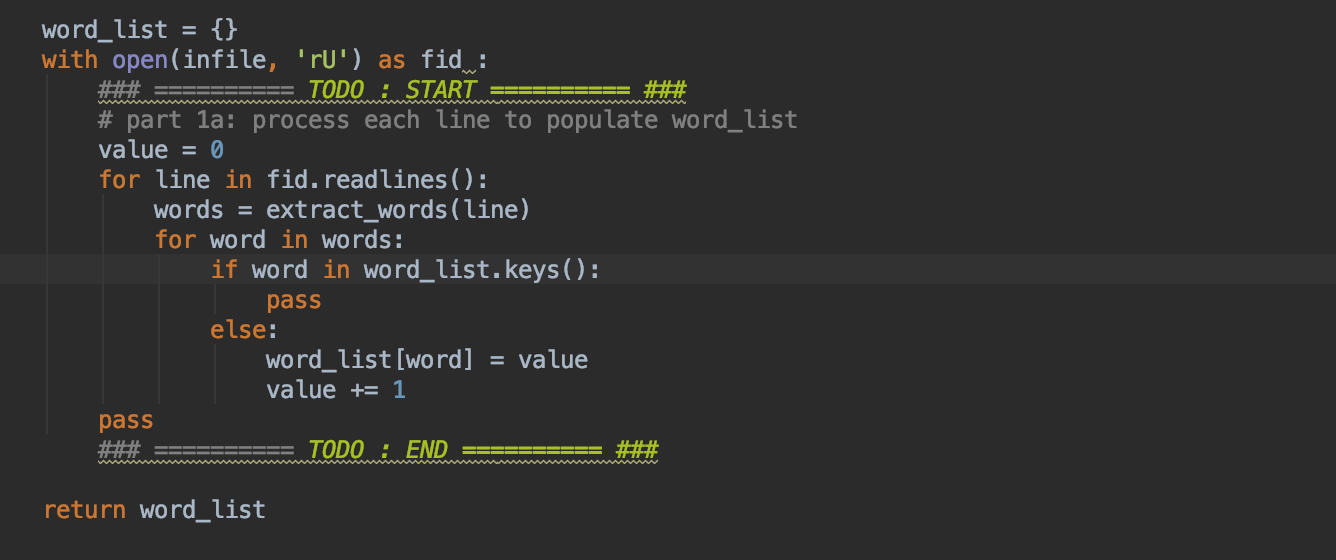
\includegraphics[width = 10cm]{4a}
	\caption{Extract word dictionary from tweets}
	\end{figure}
}

\vspace{2cm}

\item Problem 4.1(b)

\solution{
	
	\begin{figure}[h!]
	\centering
	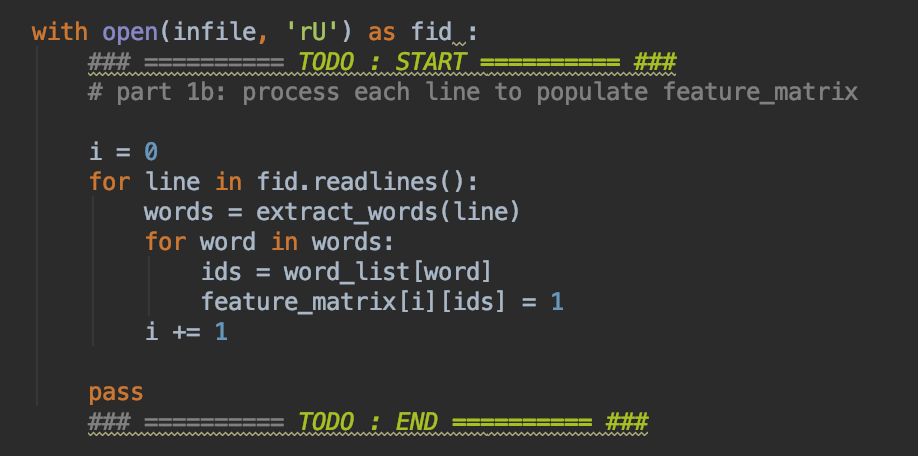
\includegraphics[width = 10cm]{4b}
	\caption{Building up feature matrix}
	\end{figure}
}

\vspace{2cm}

\item Problem 4.1(c)

\solution{
	
	\begin{figure}[h!]
	\centering
	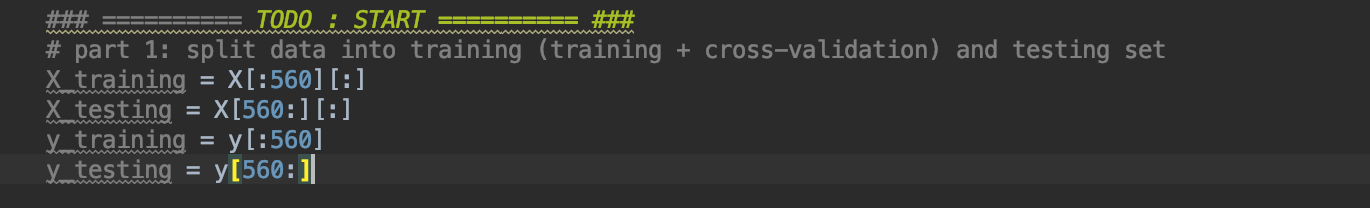
\includegraphics[width = 10cm]{4d}
	\caption{Train/test split}
	\end{figure}
	
}

\vspace{2cm}

\item Problem 4.1(d)

\solution{
	
	
	Finished feature extraction and generated train/test split

}

\end{enumerate}


\vspace{5cm}
\newpage

\section{Problem 4.2}

\begin{enumerate}

\item Problem 4.2(a)

\solution{

	\begin{figure}[h!]
	\centering
	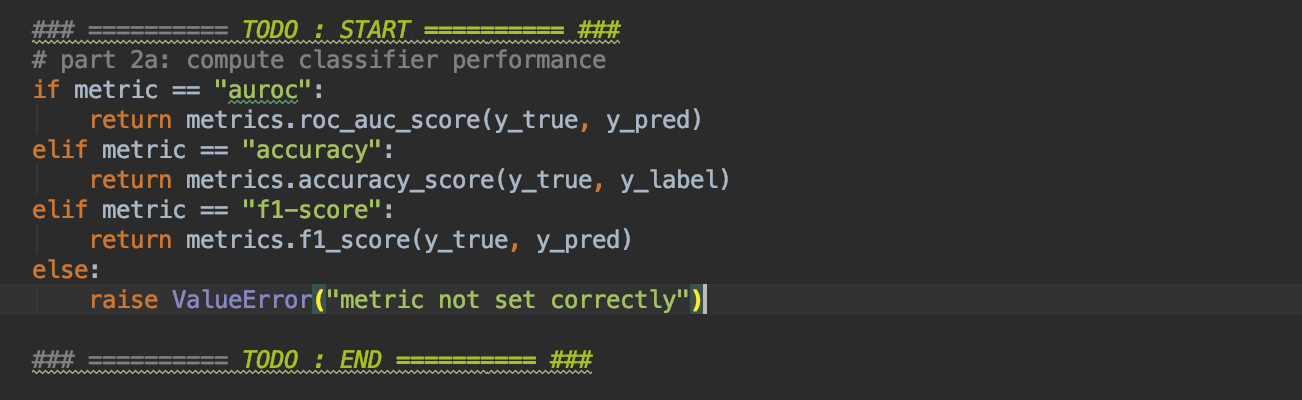
\includegraphics[width = 10cm]{4_2a}
	\caption{Implementation of performance function}
	\end{figure}
	
}

\vspace{2cm}

\item Problem 4.2(b)

\solution{
	
	\begin{figure}[h!]
	\centering
	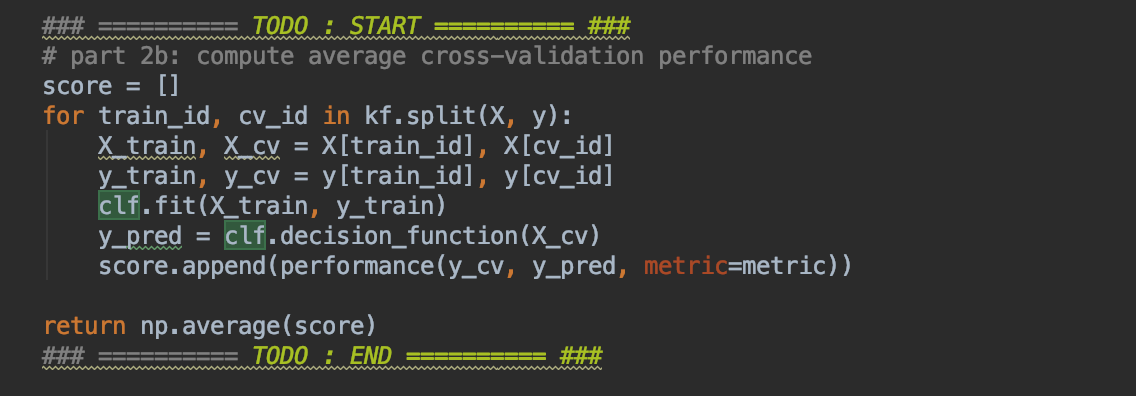
\includegraphics[width = 10cm]{42b}
	\caption{Implementation of cross validation performance function}
	\end{figure}
	
	During implementation of K-Fold validation, I used $StratifiedKFold$ to split the train and dev data in order to maintain class proportions across folds. This is important because due to the unbalance response distribution across dataset, it is possible that every train/dev split will yield a dataset from only one class, thus the model will lose generality. By using $StratifiedKFold$, we manually input some generality of the dataset as well as keep the randomness of sampling, which helps reach a balance distribution of class across folds.
	
}

\vspace{2cm}

\item Problem 4.2(c)

\solution{
	
	\begin{figure}[h!]
	\centering
	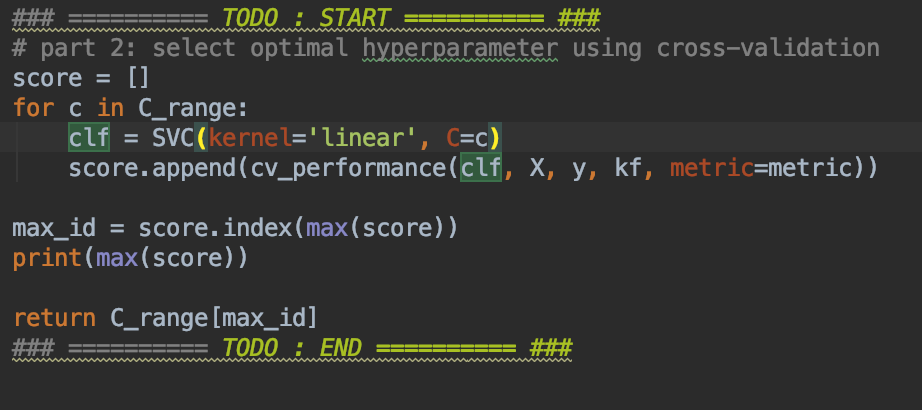
\includegraphics[width = 10cm]{42c}
	\caption{Implementation of selecting hyper parameter C}
	\end{figure}
	
}

\vspace{2cm}

\item Problem 4.2(d)

\solution{
	
	Based on ``select\_param\_ linear`` function, I found out the best setting for C for each performance measure, tabulated below:
	
	\begin{table}[h!]
	\caption{Hyper parameter C for different performance measure}
	\begin{center}
 	\begin{tabular}{||c c c c||} 
	 \hline
 	$C$ & Accuracy & F1-score & AUROC \\ [0.5ex] 
 	\hline\hline
 	$10^{-3}$ & 0.7089 & 0.8297 & 0.8106\\ 
 	\hline
 	$10^{-2}$ & 0.7107 & 0.8306 & 0.8111\\
 	\hline
 	$10^{-1}$ & 0.8060 & 0.8755 & 0.8576\\
 	\hline
 	$10^{0}$ & 0.8143 & 0.8749 & 0.8712 \\ 
	\hline
	$10^{1}$ & 0 .8182 &0.8766 & 0.8696\\
	\hline
	$10^{2}$ & 0.8182 & 0.8766 & 0.8696\\
	\hline
	Best C & $10^{1}$ & $10^{1}$ & $10^{0}$\\ [1ex]
	\hline
	\end{tabular}
	\end{center}
	\end{table}
	As we can see from the table, performances of model increases as penalty term C increases from a very small value (i.e. $10^{-2}$, $10^{-1}$), but it will remain the same if we continue to increase C after C reaches 10. In general, a large value of C suggests that model will care more about penalties and it will try to make less mistakes in training examples, but may cause overfitting while a smaller value of C suggests model cares less about making mistakes. In this example, we can see that even if we increase C from 10 to 100, none of the performance metrics increase. This suggests the training data is non-separable by using linear kernel.
}

\end{enumerate}

\vspace{5cm}

\newpage

\section{Problem 4.3}

\begin{enumerate}

\item Problem 4.3(a)

\solution{


	\begin{figure}[h!]
	\centering
	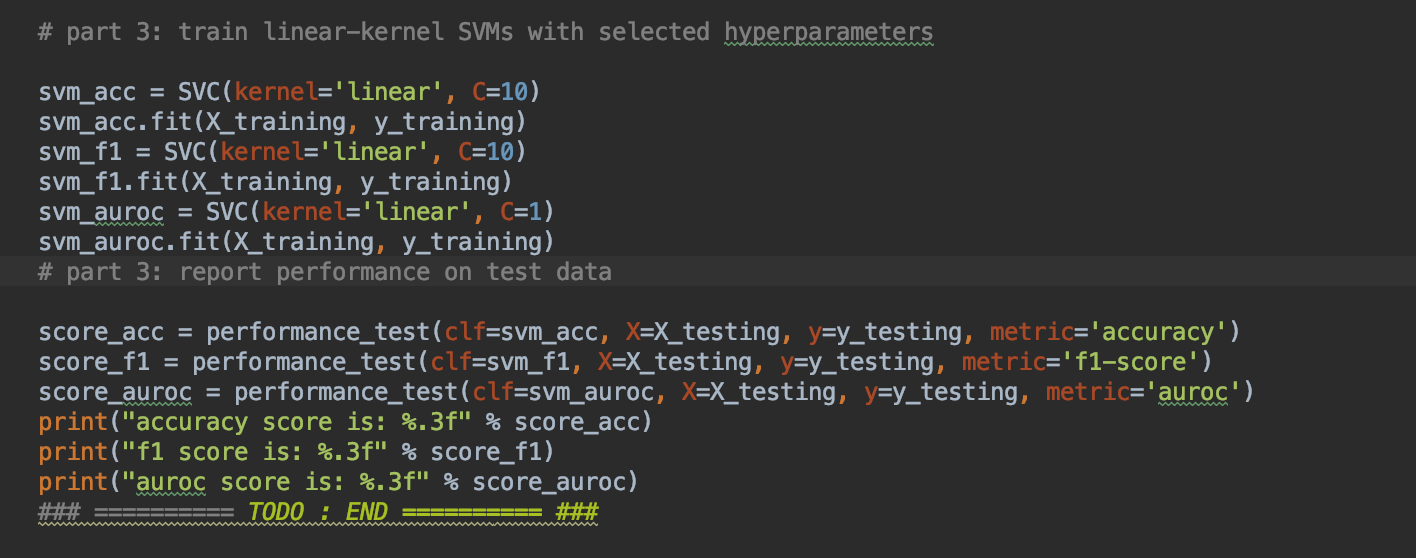
\includegraphics[width = 10cm]{43a}
	\caption{Evaluation on testing data using different metrics}
	\end{figure}

}

\item Problem 4.3(b)

\solution{
	
	\begin{figure}[h!]
	\centering
	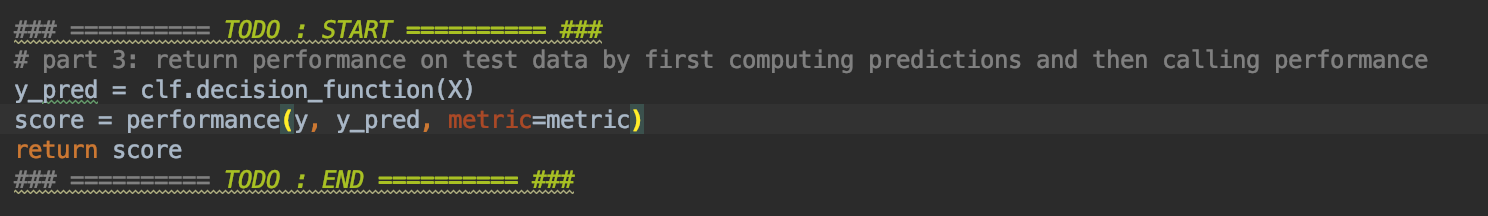
\includegraphics[width = 10cm]{43b}
	\caption{Implementation of performance test function}
	\end{figure}
	
	}
	
	
\item Problem 4.3(c)

\solution{\\
	For "accuracy", performance score is 0.743, C = 10\\
	For "f1-score", performance score is 0.437, C = 10\\
	For "AUROC", performance score is 0.741, C = 1
}

\end{enumerate}

\end{document}


\end{enumerate}

